% This is LLNCS.DEM the demonstration file of
% the LaTeX macro package from Springer-Verlag
% for Lecture Notes in Computer Science,
% version 2.4 for LaTeX2e as of 16. April 2010
%
\documentclass{llncs}
%
\usepackage{graphicx}
%\usepackage{makeidx}  % allows for indexgeneration
%
\begin{document}
%
\mainmatter              % start of the contributions
%
\title{Harnessing Wasted Computing Power for
Scientific Computing}
%
%
\author{S\'andor Guba \and M\'at\'e \H{O}ry \and Imre Szeber\'enyi}
%
\authorrunning{Ivar Ekeland et al.} % abbreviated author list (for running head)
%
%%%% list of authors for the TOC (use if author list has to be modified)
%\tocauthor{Ivar Ekeland, Roger Temam, Jeffrey Dean, David Grove,
%Craig Chambers, Kim B. Bruce, and Elisa Bertino}
%
\institute{Budapest University of Technology and Economics, Hungary,\\
\email{\{guba.sandor,orymate,szebi\}@iit.bme.hu}
}

\maketitle              % typeset the title of the contribution

\begin{abstract}

Nowadays more and more general purpose workstations installed in a student laboratory have a built in multi-core CPU and graphics card providing significant computing power. In most cases the utilization of these resources is low, and limited to lecture hours. The concept of utility computing plays an important role in technological development. 
In  this paper, we introduce a cloud management system which enables the simultaneous use of both dedicated resources and opportunistic environment. All the free workstations are to a resource pool, and can be used like ordinary cloud resources. Our solution leverages the advantages of HTCondor and OpenNebula systems.
Modern graphics processing units (GPUs) with many-core architectures have emerged as general-purpose parallel computing platforms that can dramatically accelerate scientific applications used for various simulations. Our business model harnesses the computing power of GPUs as well, using the needed amount of unused machines.
Our pilot infrastructure consists of a high performance cluster and 28 workstations with dual-core CPUs and dedicated graphics cards. Altogether we can use 10,752 CUDA cores through the network.


\keywords{Cloud, GPGPU, Grid, HTC, Utility computing}
\end{abstract}
%


\section{Introduction}
In universities there is a huge demand for high performance computing, but the smaller research groups can not afford buying a supercomputer or a large compute cluster. However significant unused computing capacity has been concentrated in the student laboratories. Most of our student labs have quite new PCs with modern multi-core CPUs and high performance graphics cards. The total computing performance of the laboratory resources could be significant. The open questions are: a) how can we collect and use these resources; b) what is the time limit of the usage; c) what happens if one or more jobs are not finishing at the given time slot; d) what management software and management rules are needed to support the various software environments which must be flexible and on demand. 

In this paper we are investigating these problems and we introduce a solution based on a new approach. We show that the cloud technology, based on hardware accelerated virtualization, can be the right answer to these questions. First of all the management of the cloud based systems are easier and they are more flexible. According to the literature\cite{younge2011analysis} and our experiences the modern virtualization has minimal overhead compared with the native systems and has more advantages than disadvantages.

Our basic idea is to run only a minimal host operating system on the bare metal and virtualize everything else. In this manner we can easily solve the questions raised up. We do not need a time consuming cloning process for the configuration management. We can save the ongoing scientific computing process at any time, and we can restore and continue it  even on another host machine. One can say, yes, these goals are solved already by various cloud management systems in corporate environment. So what is the novum on this? 

The main difference between the  corporate cloud infrastructure running 24/7 and our laboratory environment is that the corporate infrastructure is used only for serving the virtual machines. However, functions of our student laboratory are twofold:  1) During the scheduled lab exercises, the workstations act as a cloud host which serves only the virtual machines owned by the student sitting in front of the workstation or act as a simple cloud client. 2) While the lab is not used for teaching, the workstations are acting as a normal cloud host running computing intensive jobs like a normal HTCondor executing machine. 

Our solution, CIRCLE (Cloud Infrastructure for Research and Computer Labs in Education) is not only harnessing the idle CPU cycles for scientific computing, but it provides
an easy and flexible web-portal for the usage and the management as well. The user can easily manage their virtual machines and access the files stored on the online storage. Nevertheless the lecturers can easily customise a new virtual machine image and share this image with the students. In this way all the students have the same and clean learning environment which enables to concentrate on the real task. 

In the following sections we present the applied technologies and components used in our pilot system. 

\section{Virtualization}
Most IaaS (infrastructure as a service) cloud systems are based on virtual machines. Although the technique has been available since the end of 1960's\cite{creasy1981origin}, widespread adoption of x86 based systems in the server segment made it almost entirely disappear. Later some vendors started implementing different software based solutions for virtualizing operating systems or even emulating CPUs. The renaissance of virtualization began with manufacturers extending the x86 instruction set to  support low-overhead virtualization. This extension is known as Intel VT-x or AMD-V.

Current popular techniques are operating system virtualization and full hardware accelerated virtualization. The former typically takes shape in chroot environments and in namespacing of some kernel resources. This does not even allow running different kernels, nor different kinds of operating systems. The latest technique is full hardware accelerated virtualization, which is based on the CPU support for isolating the concurrently running instances. This approach is normally extended with paravirtualized device drivers, which eliminate the need for emulating real world storage and network controllers.

Hardware accelerated virtualization requires CPU support, but this is only missing currently on the low-end product line of the main x86 CPU manufacturers: some models of Intel Atom, Celeron, and Pentium. This hardware acceleration provides a near-native performance in HPC applications.\cite{younge2011analysis}

Currently there are more competing full virtualization solutions, the most notable free ones are KVM and XEN. At the time of our decision, the installation of a XEN hypervisor required modifications to the Linux kernel, and this was unacceptable for us. This is no longer the case, but we are satisfied with KVM.

Additionally, we use all KVM functions through the libvirt library, which provides an abstract interface for managing virtual machines.\cite{victoria2009creating} This has the benefit of theoretically flawless migration to other hypervisors like XEN, ESXi, or Hyper-V.\cite{bolte2010non}

Physically accessible computers are normally used with directly attached devices like display and keyboard. These devices are also emulated by KVM, and you can access virtual machines' consoles via the VNC protocol. This is useful for installing the operating system or troubleshooting, but Windows and Linux both provide better alternatives for remote access.

We use remote desktop protocol for accessing Windows hosts, and secure shell (SSH) for text-based Linux machines. Remote graphical login to X11 servers has always been available, but this is not reliable even on local network connections because it is stateless. We use instead NoMachine NX\cite{pinzari2003introduction}.
   
\section{Networking}
Most virtual machines in a cloud must have a network connection.  On the physical layer, our KVM hypervisor gives us a virtual network interface controller, which is an emulated or paravirtualized NIC on the side of the guest operating system, and a virtual NIC on the host side.

Virtual machines are connected to virtual networks provided by manageable virtual switches (Figure~\ref{fig:figure1}). The Open vSwitch.\cite{pfaff2009extending}, what we are using, is a high performance multi-layer virtual switch with VLAN, QoS and OpenFlow support, merged into the mainline Linux kernel.

Virtual networks do not necessarily differ from physical ones in the upper layers. The most important different condition is the frequency of changes. Our system in traditional physical networks' point of view is like if someone changed the cabling hundred times in the middle of the day. The developed CIRCLE networking module consists of an iptables gateway, a tinydns name server and an ISC DHCP server. All of these are configured through remote procedure calls, and managed by a relational database backed object model. 

Our solution groups the VMs to two main groups. The public vm-net is for machines which provide public services to more people, the private vm-net is for those which are used only by one or two persons. Public vm-net machines have public IPv4 and IPv6 addresses, and are protected with a simple ipset-based input filter. On the private vm-net, machines have private IPv4 and public IPv6 addresses. The primary remote connection is reached by automatically configured IPv4 port forward, or directly on the IPv6 address. As connecting to the standard port is a more comfortable solution, users who load our web portal from an IPv6 connection, get a hostname with public AAAA and private A records. If the user has no IPv6 connection, we display a common hostname with a single A record, and a custom port number. As IPv6 is widely available in the central infrastructure of our university, IPv6-capable clients are in majority. Users can open more ports, which means enabling incoming connections, and setting up IPv4 port forwarding in the background.

  \begin{figure}[ht]
    \begin{minipage}[b]{0.5\linewidth}
      \centering
      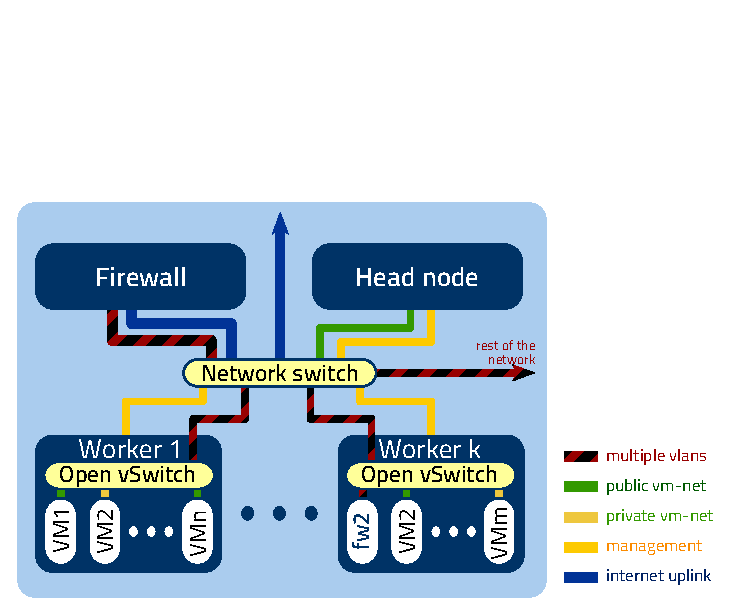
\includegraphics[width=\textwidth]{netarch}
      \caption{The structure of the network}
      \label{fig:figure1}
    \end{minipage}
    \hspace{0.5cm}
    \begin{minipage}[b]{0.4\linewidth}
      \centering
      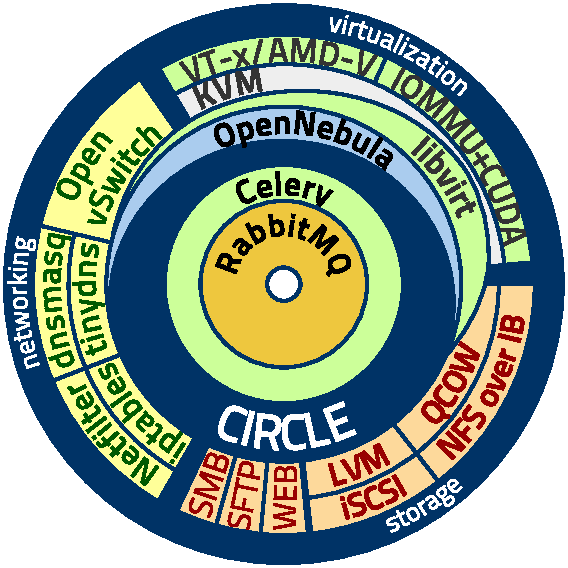
\includegraphics[width=\textwidth]{swarch}
      \caption{Technologies used for CIRCLE}
      \label{fig:figure2}
    \end{minipage}
      
  \end{figure}

\section{Storage}
Virtual machines' hard drives are provided to the hypervisors as read-write NFS shares managed by OpenNebula. Our cluster has a legacy InfiniBand SDR network, which is despite its age much faster than the gigabit Ethernet network. InfiniBand has its own data-link protocol, and Linux has mainline support for remote direct memory access (RDMA) over it , which provides near-local access times and no CPU load.\cite{callaghan2002nfs} Unfortunately this kernel module causes random cluster-wide kernel panics, which is unacceptable in a production system. We decided to use NFS4 over IP over InfiniBand, which also provided near-local timing. One problem remained: intensive random writes made the local file access on the NFS server slow (both with RDMA and IP over IB). Switching to the deadline scheduler solved this.

Disk images are stored in qcow2 (QEMU copy on write) format, which allows images with large free space to be stored in a smaller file, and also supports copy-on-write differential images. The latter feature is used for virtual machines, which eliminates the need of copying the whole base image file before launching a new instance. Saving a template consists of merging the base and differential images to a single one.

Since our usual virtual machines have temporary disks there is common need for a permanent online storage that can be easily accessed. It allows the user to use the same resources on different virtual computers or even at home, and it helps sharing data between virtual machines and local computers on a simple interface.

Our solution---CIRCLE File Server---is a multi-protocol file server, which runs on a virtual machine. Every user gets an amount of disk space, which is automatically mounted on our prepared appliances.

Windows VMs access the storage over SMB/CIFS. The authentication is handled by CIRCLE with automatically generated passwords. For security reasons we do not allow SMB access outside vm-net.
Linux guests mount the remote files with SSHFS\cite{hoskins2006sshfs}, a userspace SSH/SFTP virtual file system. For virtual machines the manager automatically generates key-pairs. SFTP service is also accessible over the internet. Users can set public keys on the web portal and immediately access their folder.

It is also possible to manage files on the cloud portal with an AJAX based web interface. Its backend consists of a Celery worker and an Nginx httpd.

\section{Putting it together}
The main goal was to give a self-service interface to our researchers, lecturers, and students.
Cloud management frameworks like OpenNebula and OpenStack promise this, but after learning and deploying OpenNebula, we found even its Self-Service portal's abstraction level too low.

Our solution is a new cloud management system, called CIRCLE, built up from various open source software components(figure~\ref{fig:figure2}). It provides an attractive web interface where users can do themselves all the common tasks including launching and managing/controlling virtual machines, creating templates based on other ones, and sharing templates with groups of users.

This cloud management system is based on Django\cite{holovaty2009definitive}. This popular Python framework gives us among other things a flexible object-relational mapping system. Although the Django framework is originally designed for web applications, the business logic is not at all web specific. That's why it is easy to provide command line or remote procedure call interfaces to the model.

As the primary interface is web, which is in some aspect a soft real-time system, the model can not use synchronous calls to external resources, nor execute system commands. This is the reason why all remote procedure calls are done asynchronously through a standard task queue. Our choice is the Celery distributed task queue. This is the most popular among such systems, which are integrated with Django. Celery is configured to use an implementation of AMQP\cite{vinoski2006advanced} protocol---called RabbitMQ---as its message broker.

Celery workers set up the netfilter firewall, the domain name and DHCP services, the IP blacklist, execute file server operations, and also communicate with OpenNebula. This distributed solution makes it possible to dynamically alter the subsystems.

In the opposite direction, some subsystems notify others of their state transitions through Celery. Based on this information further Celery tasks are submitted, and the models are updated.

CIRCLE manages the full state space of the resources. Some of it is also stored by the underlying OpenNebula, but most of this redundant information is bound to its initial value as OpenNebula does not handle changes in meta information. This behavior arises of design decisions, and is not expected to be improved. The thin slice of OpenNebula used by our system is continuously shrinking, and we intend dropping OpenNebula in favor of direct bindings to libvirt and the also considerably customized storage and network hooks.

\section{Execution on workstations}
The cloud system at our institute takes a big role in education and in general R{\&}D infrastructure, but there is a significant demand for high-throughput scientific computing. This  kind of requirement usually appears in form of many long-running, independent jobs. On most parts of the world there is no fund to build dedicated HPC clusters with enough resources for these jobs.

The highest load on the cloud takes place in the office hours and the evenings, in more than half of the time we have many free resources, so it is possible to run these jobs on low priority virtual machines in the cloud. If interactive load is increasing, we can even suspend these machines, and resume them later.

Running scientific batch jobs on student laboratory computers also has a long history. Our idea is to run some of these jobs on virtual machines in the computer laboratories overnight and on weekends. We can suspend in the morning all virtual machines to a memory image, and resume on the same or some other hypervisor next evening. This solution makes it possible to run individual jobs virtually continuously through months or a year, without any specific efforts. This result is important because of our observation that the runtime of similar jobs have a high standard deviation, and it also protects against losing the partial result of months long computations in case of hardware or power failure. HTCondor has a similar result with its checkpoint support, but it needs to modify the software, which is often impossible or sometimes the users are not able to do this modification by themselves. 

To be able to resume suspended machines, we have to copy back the differential image and the memory dump. Our choice for this is rsync.

The lab network is exposed to unauthorized access, so we have to limit access to confidential material. As a physically accessible general purpose workstation does not currently have a way to reliably authenticate itself to a server, nor to protect the stored data, we can not employ any solution against these attacks other than security through obscurity and not using these systems for any confidential executions.

Another important aspect is energy efficiency. We have successfully used HTCondor to automatically turn on and off the compute nodes of a HPC cluster. This is also working with Wake on LAN and SSH on the workstations.

\section{GPUs in the cloud}
The most significant HPC performance in our student laboratories is provided by the mid-level GPUs in all the workstations used for teaching computer graphics. There is a technology we applied successfully to use GPGPUs from the dedicated clusters' virtual machines: PCI passthrough.\cite{yang2012implementation} However, this technology requires both CPU and motherboard support of IOMMU, which is a high-end feature nowadays. The implementations are called Intel VT-d and AMD-Vi technologies, and they appear in the server- and high-end workstation segments.

As none of our laboratory computers support IOMMU, we have to find a different solution. The first one is using rCUDA, which is a small framework making it possible to run the host and device side of a CUDA program on different hosts, communicating over TCP/IP or InfiniBand network.\cite{duato2011enabling} With this, we can launch user-prepared virtual machines on each host, and run the device code via local (virtio-based) network on the hypervisor. rCUDA is also capable to serve more clients with a single device. This is useful if the host code uses the GPU only part time.

The other option is using directly the host machine to execute GPGPU jobs. This is a simpler approach, but necessarily involves a more complicated scheduler. Our choice for this type of problems is HTCondor, which can manage this scenario without much customization. The disadvantage is that the user can not customize the host-side operating system.



\section{Conclusions and future plans}
Our cloud system is built up in a modular manner. We have implemented all the main modules which enabled us to set up a production system. The system is now used as an integral part of our teaching activity, and also hosts several server functions for our department to use. At the time of writing this paper, there are 70 running and 54 suspended machines, using 109GiB of memory and producing not more than 3{\%} cummulated host cpu load on the cluster. In the first two months' production run, more than 1500 virtual machines have been launched by 125 users.

The students found the system useful and lecturers use it with pleasure because they can really set up a new lab exercise in minutes. The feedback from the users is absolutely positive, which encourages us to proceed and extend our system with the GPGPU module. We are working on making it fully functional, and releasing the whole system in an easily deployable and highly modular open source package. We are planning to finish the current development phase until the end of August. 

\emph{We thank to the other members of the developer team: D\'aniel Bach, Bence D\'anyi, and \'Ad\'am Dud\'as. }


\bibliographystyle{splncs}
\bibliography{proceedings}

\end{document}






